\section{Lezione 13 - 13/10/2023}

\subsection{Alberi Red - Black}
Gli alberi Red - Black, sono alberi binari di ricerca che associano dei colori ai loro nodi. 
%Come ogni tipo di struttura dati ha le sue caratteristiche. 
La colorazione ovviamente andrà a braccetto con alcune proprieta (vincoli) che di seguito andremo a definire.

\begin{itemize}	
	\item[1)] Ogni nodo deve essere rosso o nero.
	\item[2)] \textbf{I nodi foglie possono essere solo neri (NIL)}, quindi i nodi rossi potranno essere soltanto all'interno. 
	\item[3)] Ogni nodo rosso ha \textbf{solo} figli neri.
	\item[4)] Per ogni nodo X preso all'interno dell'albero, ogni percorso da X al nodo foglia contiene \textbf{lo stesso numero} di nodi neri.
\end{itemize}

\begin{figure}[H]
	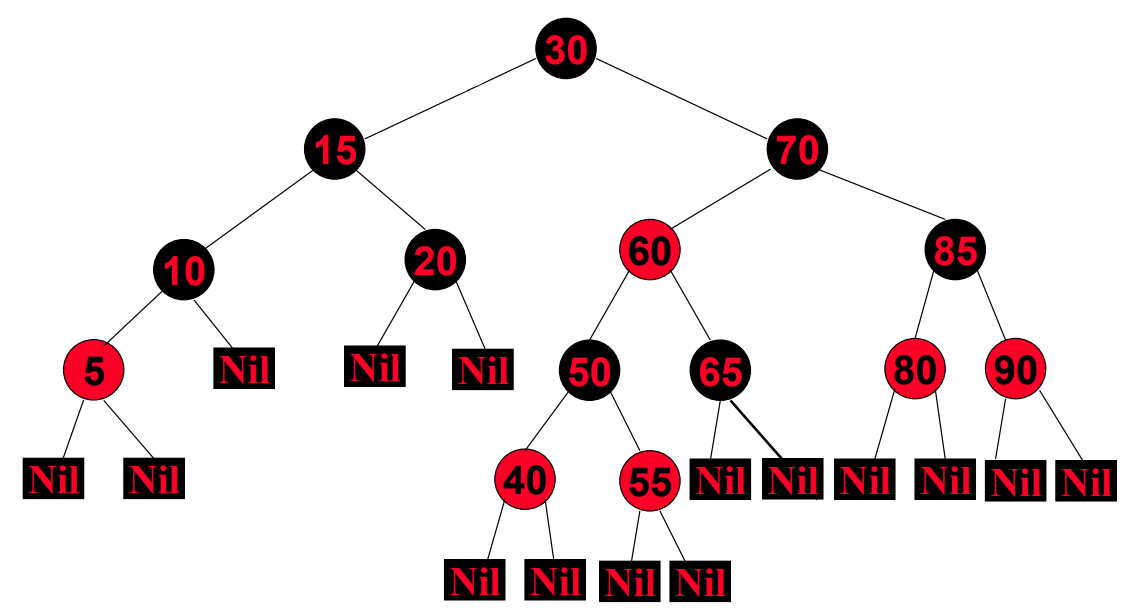
\includegraphics[width=\textwidth]{AlberoRB} 
	\caption{Questo è un albero RB perché soddisfa tutti e 4 i vincoli}
\end{figure}

\paragraph{Non tutti gli alberi possono essere colorabili}
\mbox{}
\smallskip

Per vedere se un albero è colorabile ci sono delle considerazioni da fare:

\begin{itemize}
    \item Colorare subito le foglie e la radice di nero.
    \item Osservare se esiste un sottoalbero è visibilmente piu pesante di un altro. In tal caso l'albero è quasi sicuramente non colorabile. Teoricamente se la differenza di altezza di alberi è maggiore di due allora probabilmente non è colorabile.
\end{itemize}

\subsubsection{Altezza Nera di un albero R-B}
L'altezza nera, di un albero R-B, è il numero di nodi neri che, preso un nodo X, si contano da X fino alle foglie escludendo X.

L'altezza nera è sicuramente minore dell'altezza dell'albero e al massimo uguale.

Dimostriamo dunque che l'altezza è sicuramente:

$$h \le 2^{bh(x)}-1$$

Preso un nodo all'interno di un albero il numero di nodi interni non può essere più piccolo di un albero completamente nero.
$$ n i(x) \ge 2^{bh(x)} -1 $$

Dimostriamo per induzione

\begin{itemize}
	\item Base Induttiva: Albero di altezza zero, quindi il numero di nodi interni di un albero di $h=0$ è \textbf{zero}, andiamo a svolgere l'equazione con la base induttiva:
	$$ 0 \ge 2^{bh(x)}-1 \Rightarrow 2^0-1 = 0 \Rightarrow \text{ VERO }$$
	
	
	\item Caso Induttivo $h > 0$: L'albero contiene almeno un nodo interno. 
	Andiamo a scomporre il nostro albero come sottoalbero sx del figlio sinistro e sottoalbero dx del figlio destro.
	$$ ni(y) \ge 2^{bh(y)}-1 $$
	$$ ni(z) \ge 2^{bh(z)}-1 $$
	Noi sappiamo che 
	$$ ni(x)=1+ni(y)+ni(z) $$
	
	In questo caso, ragionando analiticamente possiamo dire che l'altezza nera di X, il nostro nodo padre del sottoalbero dipende dal fatto che y, il suo sottoalbero sinistro, sia nero o rosso.
	\begin{itemize}
		\item Nel caso in cui il nodo sia rosso, allora l'altezza nera di x e y sono uguali.
		\item Nel caso in cui il nodo sia nero, allora l'altezza nera di x e uguale a quella di y + 1.
	\end{itemize}
	
	Esplicitiamo $bh(y)$ dalle due equazioni perche ci interessa esplicitare tutto per $bh(x)$

	In questo caso vedremo che $bh(y) > bh(y) - 1$ poiche o e uguale, o e sicuramente maggiore di $bh(x) - 1$.
	
	Questo vale anche per z, dunque avremo:
	
	$$bh(y) \ge bh(x) -1$$
	$$bh(z) \ge bh(x) -1$$

	Questo vuol dire che scendendo di altezza, andro a diminuire al massimo di uno l'altezza del sottoalbero. Grazie a queste equazioni possiamo ritornare a ritroso alla tesi.
	

	Usiamo questo ragionamento matematico: Se io so che $n \ge m$, allora avro anche che $ 2^{n} \ge 2^{m}$ poiche l'esponenziale e crescente e non andiamo a modificare il risultato comunque finale. 
	
	Applichiamo dunque la stessa proprieta alle stesse equazioni scritte sopra. In tal caso avremo 
	
	$$bh(y) \ge bh(x) -1 \rightarrow 2^{bh(y)} \ge 2^{bh(x)-1} $$
	sottraiamo una stessa quantita a entrambi i membri
	$$2^{bh(y)}-1  \ge 2^{bh(x)-1}$$
	Dunque entrambi vedremo che la somma tra $2^{bh(y)} e 2^{bh(z)}$ sono maggiori o uguali di $2^{bh(x)-1}$.
	
	Il numero di nodi interni di X e dato da $1 + ni(y)+ ni(z)$. Sostituendo abbiamo che $1 + 2^{bh(x) - 1} -1 + 2^{bh(x)-1}-1 \rightarrow 2*2^{bh(x)-1}$. Il "-1" puo essere semplificato portando dentro il 2 moltiplicato avanti all'espressione. In tal modo avremmo che indipendentemente dall'altezza che io ho in entrata, il numero di nodi interni di quel sottoalbero e almeno uguale a $2^{bh(x)}-1$, quindi la tesi inziale e dimostrata.
	
	
\end{itemize}

\subsubsection{Considerazioni sull'altezza nera di un albero}

Se sappiamo che il numero di nodi n e maggiore o uguale a $2^bh -1$, possiamo intuitivamente e approssimativamente andare a trovare l'altezza nera dell'albero.

Nel caso in cui avesse tutti i nodi neri allora l'altezza nera e $\le h$, mentre se ha alternati rossi e neri, abbiamo il limite minimo dell'altezza nera, cioe $\frac{h}{2}$.

Dunque l'altezza nera e compresa tra : $\frac{h}{2} \le bh \le h$.

Usando la matematica e le nozioni della dimostrazione precedente...
$$bh \ge \frac{h}{2} \rightarrow 2^{bh} -1 \ge 2^{\frac{h}{2}-1}$$
Se sappiamo che n e $\ge 2^{bh}-1$ allora,
$$n \ge 2^{\frac{h}{2}-1}$$
$$n+1 \ge 2^{\frac{h}{2}}$$
$$\log_{2} h+1 \ge \frac{h}{2}$$
$$h \ge 2\log_{2} n+1$$

\subsubsection{Inserimento Albero R-B}
Gli algoritmi di inserimento e bilanciamento usati fino ad ora non andranno più bene per questo tipo di struttura. Nonostante abbiamo più libertà da un certo punto di vista, dobbiamo considerare che la proprieta 4 degli alberi Red-Black ci impedisce di fare degli inserimenti nella struttura dati in modo efficiente.
\smallskip

In particolare nell'inserimento di un valore in un nodo NIL, l'algoritmo deve occuparsi di creare il nodo, colorarlo e di creare e colorare a sua volta i figli NIL (di nero ovviamente).
\smallskip

Successivamente la colorazione del nodo k non è immediata e semplice, va considerato il colore del padre e non va rotto il vincolo dello stesso numero di nodi neri per ogni percorso dei sottoalberi.
\smallskip

Abbiamo due possibilità di colore all'inserimento. Solitamente per non creare problemi con il padre del sottoalbero a cui dobbiamo inserire, si inserisce nero. Anche in quel caso non e detto che l'inserimento del nero non abbia creato problemi per la proprieta 4 dei R-B.

Nei Red - Black la violazione di una di questi due algoritmi puo essere scoperta solo ricorsivamente.

\begin{lstlisting}[language=Java]
	InsertRB(T,k)
		if T != NIL then
			if T->key < k then
				T->dx = InsertRB(T->dx, k)
				T = BilanciaRBdx(T)
			else if T->key > k then
				T->sx = InsertRB(T->sx, k)
				T = BilanciaRBsx(T)
			else
				T = new_nodeRB(k,r) //Creazione nodo rosso (r) e figli a NIL
		return T
\end{lstlisting}

Questa funzione verra supportata dalle funzioni di bilanciamento che sono specificatamente scritte apposta per la R-B. In tal caso abbiamo 3 casistiche generali di problemi.
Nel caso in cui il nodo che andiamoa  inserire sia rosso...

\begin{itemize}
	\item Caso 1) Il padre rosso e il fratello rosso. Sia a destra che a sinistra del padre rosso.
	\item Caso 2) Inserimento a destra del sottoalbero il cui padre e rosso e il fratello nero.
	\item Caso 3) Inserimento a sinistra del sottoalbero il cui padre e rosso e il fratello e nero.
\end{itemize}

La risoluzione del Caso 1, si scambia il nodo padre rosso con il nonno nero, in tal caso abbiamo che i figli diventeranno perforza di cose neri. In questo modo non andiamo a violare la proprieta 4, poiche i percorsi sia a destra che a sinistra avranno lo stesso numero di nodi neri, ma andiamo soltanto ad aumentare l'altezza nera.

Il Caso 2 si risolve ruotando in modo tale da arrivare al caso 3.

Per il caso 3 ci conviene ruotare l'albero a destra e sostituire il nodo radice (precendetemente nero) con un nodo rosso (visto che era figlio di nero). In tal modo abbiamo la radice nera, i figli rossi e i sottoalberi non cambiano.

Aggiustare assolutamente